% =============================================================================
% IEEE conference-paper version of the proposal
% "Context-Aware Restaurant Recommendation with Taichung Bus Accessibility"
%
% Build (from ieee_latex/):  pdflatex ieee_paper && bibtex ieee_paper
%                           && pdflatex ieee_paper && pdflatex ieee_paper
% Requires IEEEtran.cls / IEEEtran.bst (included in TeX Live / MacTeX / Overleaf).
% For an IEEE journal, change [conference] to [journal] and adjust the author block.
% =============================================================================
\documentclass[conference]{IEEEtran}
\IEEEoverridecommandlockouts

\usepackage{cite}
\usepackage{CJKutf8}
\usepackage{amsmath,amssymb,amsfonts}
\usepackage{algorithm}
\usepackage{algpseudocode}
\usepackage{graphicx}
\usepackage{textcomp}
\usepackage{xcolor}
\usepackage{array}
\usepackage{booktabs}
\usepackage{url}
\usepackage{tikz}
\usetikzlibrary{arrows.meta,shapes.geometric}

% Colours shared with the thesis figures (figures/ch4_styles.tex)
\definecolor{archLLM}{HTML}{DCE9F8}
\definecolor{archLLMd}{HTML}{2F6DB5}
\definecolor{archPro}{HTML}{E6F2E6}
\definecolor{archProd}{HTML}{3C8D4F}
\definecolor{archKB}{HTML}{FFF3D6}
\definecolor{archKBd}{HTML}{C58A12}
\definecolor{archSrc}{HTML}{FDE9DC}
\definecolor{archSrcd}{HTML}{D9622B}
\definecolor{archGray}{HTML}{4A4A4A}

\newcolumntype{L}[1]{>{\raggedright\arraybackslash\hspace{0pt}}p{#1}}
\algrenewcommand\algorithmicrequire{\textbf{Input:}}
\algrenewcommand\algorithmicensure{\textbf{Output:}}

\begin{document}

\title{Context-Aware Restaurant Recommendation with\\Taichung Bus Accessibility}

% Authors (team members of the original proposal).
% Chinese names are typeset with CJKutf8 (pdflatex). If the venue requires
% romanized names, replace them, e.g. Yu-Chieh Wei (魏郁倢).
% TODO: confirm department and e-mail addresses.
\author{
\IEEEauthorblockN{\begin{CJK}{UTF8}{bkai}林晉德、顧晏哲、魏郁倢、葉純宇\end{CJK}}
\IEEEauthorblockA{\textit{Department of Computer Science and Engineering} \\
\textit{National Chung Hsing University}\\
Taichung, Taiwan}
}

\maketitle

% -----------------------------------------------------------------------------
\begin{abstract}
For a date, a birthday celebration, or a gathering with friends, a good restaurant must both suit the dining occasion and be practical to reach. Semantic relevance between restaurant reviews and the occasion, however, says nothing about transportation: long walks, long waits, or several transfers can make a relevant restaurant unusable, and attaching a route only after the restaurant has been chosen prevents transportation from influencing the choice. This paper proposes a context-aware restaurant recommendation agent that brings Taichung bus accessibility into the final selection. A language model converts the user's request into a fixed schema; keyword, vector, or hybrid retrieval aligns the dining context with review text and recalls a candidate set; and a knowledge graph links restaurants, attributes, and source snippets. For each candidate, itineraries and arrival estimates from the Taiwan Transport Data eXchange (TDX) are used to build a timeline of walking, waiting, riding, transfer, arrival, and dining. Budget, opening hours, boarding, and transfer constraints are checked programmatically with a three-valued verdict (pass, fail, unknown), so missing evidence is never presented as confirmed feasibility. Verified restaurants are ranked by combining contextual relevance with transportation burden, keeping only the best itinerary per restaurant. We describe the system design and a pre-registered evaluation protocol with baselines, metrics, and statistical tests; experiments are ongoing and no empirical results are reported here.
\end{abstract}

\begin{IEEEkeywords}
restaurant recommendation, review semantics, context-aware recommendation, public transport, hybrid retrieval, knowledge graph, three-valued constraint checking
\end{IEEEkeywords}

% -----------------------------------------------------------------------------
\section{Introduction}

\IEEEPARstart{E}{ating} out is a routine decision with many options. A 2025 report by the Taichung City Government counted 22{,}612 food-service businesses in the city at the end of 2024, an increase of 47.55\% over 2015~\cite{taichung_eat_outside}. Faced with this choice, users planning a date, a birthday, or a gathering need to know which restaurants actually fit the purpose of the meal. Reviews often carry such information in phrases like ``good for chatting'' or ``romantic atmosphere,'' which rarely share vocabulary with the user's request and therefore call for semantic matching. Work on subjective attributes and critique-based conversational recommendation shows the value of natural-language preferences and review evidence for this purpose~\cite{subjective_attributes,critique_preference}.

The user must also be able to get there. We study the case of diners travelling by bus in Taichung, where a trip involves walking to a stop, waiting, riding, possibly transferring, and walking to the restaurant\footnote{A 2026 city bulletin, based on 2024 survey data, reports that buses and coaches account for 3.9\% (men) and 6.0\% (women) of trips~\cite{taichung_gender}; the category covers several coach services and is not identical to urban buses.}. Consider the request ``a birthday dinner with friends tonight, under NT\$600 per person, by bus from Taichung Station.'' The system must first understand the occasion and find restaurants whose reviews support it, and then decide which of them are reachable under the user's time and transfer constraints. Ranking only by semantic relevance does not guarantee convenient access, while choosing the nearest restaurant ignores the occasion. Language-driven planning with formal verification~\cite{llm_planning_tools} and timetable-based transit routing~\cite{bus_dynamic_replanning} provide the technical ingredients, but how transportation should feed back into the choice of restaurant remains open.

This paper addresses the following problem: \emph{given a set of restaurants that match the dining context, how can bus accessibility be used to filter and rank them so that the final recommendation is both suitable for the occasion and convenient to reach, and how should unknown store or transit data be presented so that the explanation never claims more than the evidence supports?}

We propose a context-first recommendation agent in which transportation analysis happens \emph{before} the final ranking. Our contributions are:
\begin{enumerate}
\item A retrieval pipeline that aligns dining contexts with review semantics and keeps a link from every recommendation back to concrete review evidence.
\item A transportation stage that, for every candidate restaurant, compares walking, waiting, riding, and transfer burden on Taichung buses and lets this burden affect the restaurant ranking.
\item A three-valued constraint checker over a complete trip timeline for budget, opening hours, boarding, and transfers, which separates ``infeasible'' from ``insufficient evidence.''
\item Recommendation explanations generated from decision records, and an evaluation protocol designed to test whether each component actually improves recommendations.
\end{enumerate}

We do not claim that vector retrieval, knowledge graphs, or bus routing are new algorithms; the contribution lies in how they are integrated and in the domain-specific evaluation. We study four research questions:
\begin{itemize}
\item \textbf{RQ1:} Does vector or hybrid retrieval align occasions such as dates or birthdays with restaurant reviews better than keyword retrieval?
\item \textbf{RQ2:} Does filtering and ranking candidates by bus accessibility balance occasion fit and travel convenience better than semantic ranking with a route appended afterwards?
\item \textbf{RQ3:} Do three-valued checking and source/time records reduce constraint violations and unsupported claims of feasibility?
\item \textbf{RQ4:} Does a complete timeline, compared with checking opening hours at departure time or using a single API time, avoid missed boardings, broken transfers, and meals that run past closing time?
\end{itemize}

The rest of the paper is organized as follows. Section~\ref{sec:related} reviews related work. Section~\ref{sec:problem} formalizes the problem, Section~\ref{sec:method} presents the system, Section~\ref{sec:eval} describes the evaluation protocol, Section~\ref{sec:discussion} discusses design trade-offs and limitations, and Section~\ref{sec:conclusion} concludes.

% -----------------------------------------------------------------------------
\section{Related Work}\label{sec:related}

\begin{table*}[!t]
\centering
\caption{Article Summary Table}
\label{tab:article_summary}
\scriptsize
\renewcommand{\arraystretch}{1.12}
\setlength{\tabcolsep}{3pt}
\begin{tabular}{@{}L{0.65cm}L{0.7cm}L{1.9cm}L{2.1cm}L{2.0cm}L{2.4cm}L{3.0cm}L{3.15cm}@{}}
\toprule
\textbf{Ref.} & \textbf{Year} & \textbf{Problem} & \textbf{AI Method} & \textbf{Domain Knowledge} & \textbf{Dataset} & \textbf{Findings} & \textbf{Limitation} \\
\midrule
\multicolumn{8}{@{}l}{\textit{AI techniques}} \\
\cite{llm_planning} & 2024 & Multi-constraint travel planning & Language agents with tool use (benchmark) & Travel arrangements and constraints & TravelPlanner, 1,225 planning intents & GPT-4 final pass rate of 0.6\% in the two-stage setting & Commonsense criteria set by author consensus; not all users' judgments covered \\
\cite{llm_planning_tools} & 2025 & Verifiable constrained planning & LLM translates requests into formal constraints for solvers & Travel conditions; diagnosis of unsatisfiable constraints & TravelPlanner; authors' international travel dataset & 93.9\% success rate in its setting & Prompt and encoding design is costly; solver may time out; cannot detect erroneous or unsafe data \\
\cite{ttg} & 2024 & Solving natural-language travel requests & Fine-tuned LLM and mixed-integer linear programming & Flights, hotels, and attractions & Synthetic data built from real statistics & About 91\% exact match in back-translation; user study & Feasibility and optimality assume correct parsing; personalization and multi-turn dialog remain open \\
\cite{bright} & 2025 & Reasoning-intensive retrieval & Evaluation of BM25, dense, and other retrievers & Multi-domain reasoning queries & BRIGHT, 1,384 queries & Reasoning-intensive retrieval remains challenging & Relevance labels are subjective; multimodal retrieval not covered \\
\cite{hybrid_retrieval} & 2023 & Complementarity of sparse and dense retrieval & Hybrid retrieval training objectives & General information retrieval & MS MARCO, Natural Questions, TREC Robust04 & Complementarity objectives improve retrieval & Sparse labels may cause false negatives; MS MARCO biased toward exact matching \\
\cite{knowledge_graph_llm_recommendation} & 2025 & Knowledge support for LLM-based recommendation & K-RagRec & Movie and book recommendation & MovieLens, Amazon Book & Structured knowledge improves recommendation; hallucinated items analyzed & Only 7B/8B models and Freebase evaluated; popularity-based retrieval policy \\
\midrule
\multicolumn{8}{@{}l}{\textit{Restaurant and bus domain knowledge}} \\
\cite{subjective_attributes} & 2022 & Expressing subjective attributes & Conceptual framework & Perspective and subjectivity in recommendation language & None (position paper) & Outlines problems and research directions & Preliminary framework; formal semantics, methods, and metrics left open \\
\cite{critique_preference} & 2021 & Turning restaurant critiques into preferences & LM transformation, embeddings, review ranking & Dining atmosphere and preference revision & Restaurant critiques and reviews & Ablation shows critique transformation improves recommendation & Excluding unsuitable restaurants via critiques and clarifying critique scope left open \\
\cite{restaurant_habib} & 2016 & Location-, time-, and preference-aware restaurant recommendation & Time decay, mutual reinforcement, product scoring & Distance, check-in-based active hours, popularity & Foursquare Paris: 7,991 restaurants, 111,325 check-ins, 6,903 users & Two example queries show the effect of preference and meal time & No customer reviews; illustrative queries only, no aggregate accuracy or significance test \\
\cite{poi_stisan} & 2022 & Next-POI recommendation & STiSAN spatio-temporal attention & Spatio-temporal visit intervals & Gowalla, Brightkite, Weeplaces, Changchun & Evaluates interval modeling for sequential recommendation & TAAD helps only in some cases, possibly because the last-POI--candidate spatial interval is ignored \\
\cite{bus_dynamic_replanning} & 2025 & Dynamic replanning in public transport & Connection scan, relevant timetable range, push/pull updates & Trips, transfers, walking, delays & GTFS networks of Perth, Berlin, Paris, London; synthetic delays & Better arrival times and lower update query load in simulation & Synthetic delays; real-delay validation and multicriteria routing left open \\
\cite{bus_delay_uncertainty} & 2022 & Bus delays and prediction uncertainty & Student-t model, Bayesian inference & Waiting reliability, time of day, inter-stop relations & Stockholm high-frequency bus data & Probabilistic delay prediction; Student-t outperforms Gaussian & Broader data needed for network and high/low-frequency effects; possible overparameterization at end-of-route stops \\
\bottomrule
\end{tabular}
\end{table*}

\subsection{Language-Driven Planning with Verification}
TravelPlanner evaluates language agents on 1{,}225 planning intents and shows that multi-constraint, long-horizon planning remains hard; GPT-4 reached a final pass rate of only 0.6\% in its two-stage setting~\cite{llm_planning}. Hao \emph{et al.} translate requirements into formal constraints solved by external tools, reaching a 93.9\% success rate in their TravelPlanner setting, while noting that prompt design, solver runtime, and errors in the underlying data remain open issues~\cite{llm_planning_tools}. TTG similarly maps natural language to a symbolic form solved by mixed-integer linear programming~\cite{ttg}, whereas HyperTree Planning improves the planning ability of the model itself through hierarchical decomposition~\cite{hypertree_planning}. Because models, tools, and evaluation settings differ across these papers, their success rates cannot be compared directly. We adopt the division of labour in which the language model parses input and code checks constraints, because our constraints must be traceable and applied consistently, not because model-side planning is ineffective.

\subsection{Semantic Retrieval and Structured Evidence}
BRIGHT shows that reasoning-intensive queries remain difficult for both lexical and dense retrievers~\cite{bright}, so we cannot assume that embeddings dominate keywords for every query. Hybrid retrieval exploits the complementarity of sparse and dense signals~\cite{hybrid_retrieval}. We therefore compare BM25, vector, and hybrid recall, so that both semantic preferences (``good for groups'') and exact terms (place or dish names) are covered. K-RagRec retrieves structured knowledge-graph evidence to support LLM-based recommendation of movies and books~\cite{knowledge_graph_llm_recommendation}. We borrow the idea of evidence-backed recommendation but treat \emph{storing evidence} and \emph{using a graph} as separate factors to be tested.

\subsection{Subjective Preferences, Location, and Time}
Radlinski \emph{et al.} point out that the same description can be read differently by different users~\cite{subjective_attributes}, and Bursztyn \emph{et al.} transform restaurant critiques into positive preferences used to retrieve supporting reviews~\cite{critique_preference}. Both support keeping the original wording and source snippets instead of treating atmosphere labels as objective facts. Habib \emph{et al.} combine current location, request time, check-in history, and popularity to recommend restaurants on a Foursquare Paris subset, but do not use customer reviews and report only illustrative queries~\cite{restaurant_habib}. STiSAN models spatio-temporal intervals for next-POI recommendation~\cite{poi_stisan}. These works show that location and time matter, yet similarity of preference does not imply that a user can arrive and finish a meal; we handle preference in ranking and feasibility in checking.

\subsection{Public Transport Timing and Uncertainty}
Bus feasibility depends on the order of events: a vehicle that has left before the user reaches the stop cannot be boarded even if the API reports normal service, and a transfer requires arriving, walking, and buffering before the next departure. Abuaisha \emph{et al.} model trips with connections, transfers, and footpaths and compare push- and pull-based replanning on GTFS networks of Perth, Berlin, Paris, and London using synthetic delays~\cite{bus_dynamic_replanning}. Rodriguez-Deniz and Villani model Stockholm bus delays with Student-t distributions and Bayesian inference, showing that point estimates hide substantial uncertainty~\cite{bus_delay_uncertainty}. TDX provides trip-planning and bus data APIs for Taiwan~\cite{tdx_planner,tdx_bus}.

\subsection{Article Summary}
Table~\ref{tab:article_summary} summarizes six studies on AI techniques and six on restaurant and bus domain knowledge, together with the limitations stated by their authors.


\subsection{Research Gap}
Existing work provides semantic retrieval, subjective preference modelling, spatio-temporal recommendation, and transit routing, but separately: restaurant recommenders ask whether a place fits, and transit planners ask how to get there. To our knowledge, no prior study recalls occasion-matched restaurants from reviews and then filters and ranks them by bus walking, waiting, riding, and transfer conditions while explicitly representing missing evidence. We position this work as an integration and domain-validation study rather than claiming that no related work exists.

% -----------------------------------------------------------------------------
\section{Problem Formulation}\label{sec:problem}

The input is a natural-language request together with an origin and a departure time; the output is at most three distinct restaurants, each with its contextual evidence and a recommended bus itinerary. The decision unit is the \emph{restaurant}. A pair $z=(r,p)$ of restaurant $r$ and itinerary $p$ is used only for computation and checking.

A request is represented as
\begin{equation}
q=(c,\,o,\,t_{\mathrm{dep}},\,B,\,L_{\max},\,W_{\max},\,N_{\max},\,D_{\mathrm{meal}}),
\end{equation}
where $c$ is the dining context, $o$ the origin, $t_{\mathrm{dep}}$ the departure time, $B$ the budget in a declared unit (per person or per group), $L_{\max}$ the walking limit (per leg or in total, as specified by the user), $W_{\max}$ the waiting limit, $N_{\max}$ the maximum number of transfers, and $D_{\mathrm{meal}}$ the meal duration. Relative times are resolved to absolute dates, and missing or ambiguous key fields trigger a clarification question.

Requirements fall into three classes: \emph{contextual preferences} (e.g., ``date,'' ``birthday''), used for semantic recall and ranking; \emph{hard constraints} (budget, opening hours, walking and transfer limits), checked against evidence; and \emph{dynamic states} (bus ETA, arrival time), used to build the timeline. From the corpus $\mathcal{D}$, the system recalls a restaurant set $\mathcal{R}_K(q)$ and, for each $r\in\mathcal{R}_K(q)$, obtains itineraries $\mathcal{P}(r,o,t_{\mathrm{dep}})$. Semantic recall thus defines the search space, and transportation analysis determines feasible itineraries and the final order within it. Text from external sources is treated as evidence only and has no authority to change system rules or trigger tools.

% -----------------------------------------------------------------------------
\section{Proposed System}\label{sec:method}

\subsection{Design Principles}
(i) Find context-matching restaurants first and plan transport second, so that convenience never promotes clearly unsuitable restaurants. (ii) Analyse transport \emph{before} the final ranking. (iii) Check hard constraints in code; a high semantic score cannot offset a known violation. (iv) Express uncertainty when evidence is insufficient. (v) Make every explanation traceable to reviews, data, and decision records.

\subsection{Architecture}
Fig.~\ref{fig:architecture} shows the nine modules. Modules 1--3 prepare data offline: (1) collecting reviews, video transcripts, and store information; (2) extracting restaurant entities, branches, context snippets, prices, and hours with manual verification; and (3) storing snippets in a vector index and restaurants, attributes, and evidence relations in a knowledge graph and relational tables. Modules 4--9 form the online pipeline: (4) an LLM parses the request into the schema, and a programmatic planner validates input and orchestrates tools; (5) retrieval aligns the context with reviews and deduplicates by restaurant; (6) evidence lookup removes candidates already known to violate itinerary-independent constraints such as budget; (7) TDX itineraries and arrival data are used to analyse walking, waiting, riding, and transfers; (8) three-valued checking and ranking select the best itinerary per restaurant and order restaurants; and (9) the output presents restaurants, review evidence, transport burden, and unknown items, and lets the user revise the request.

\begin{figure*}[t]
\centering
\resizebox{\textwidth}{!}{%
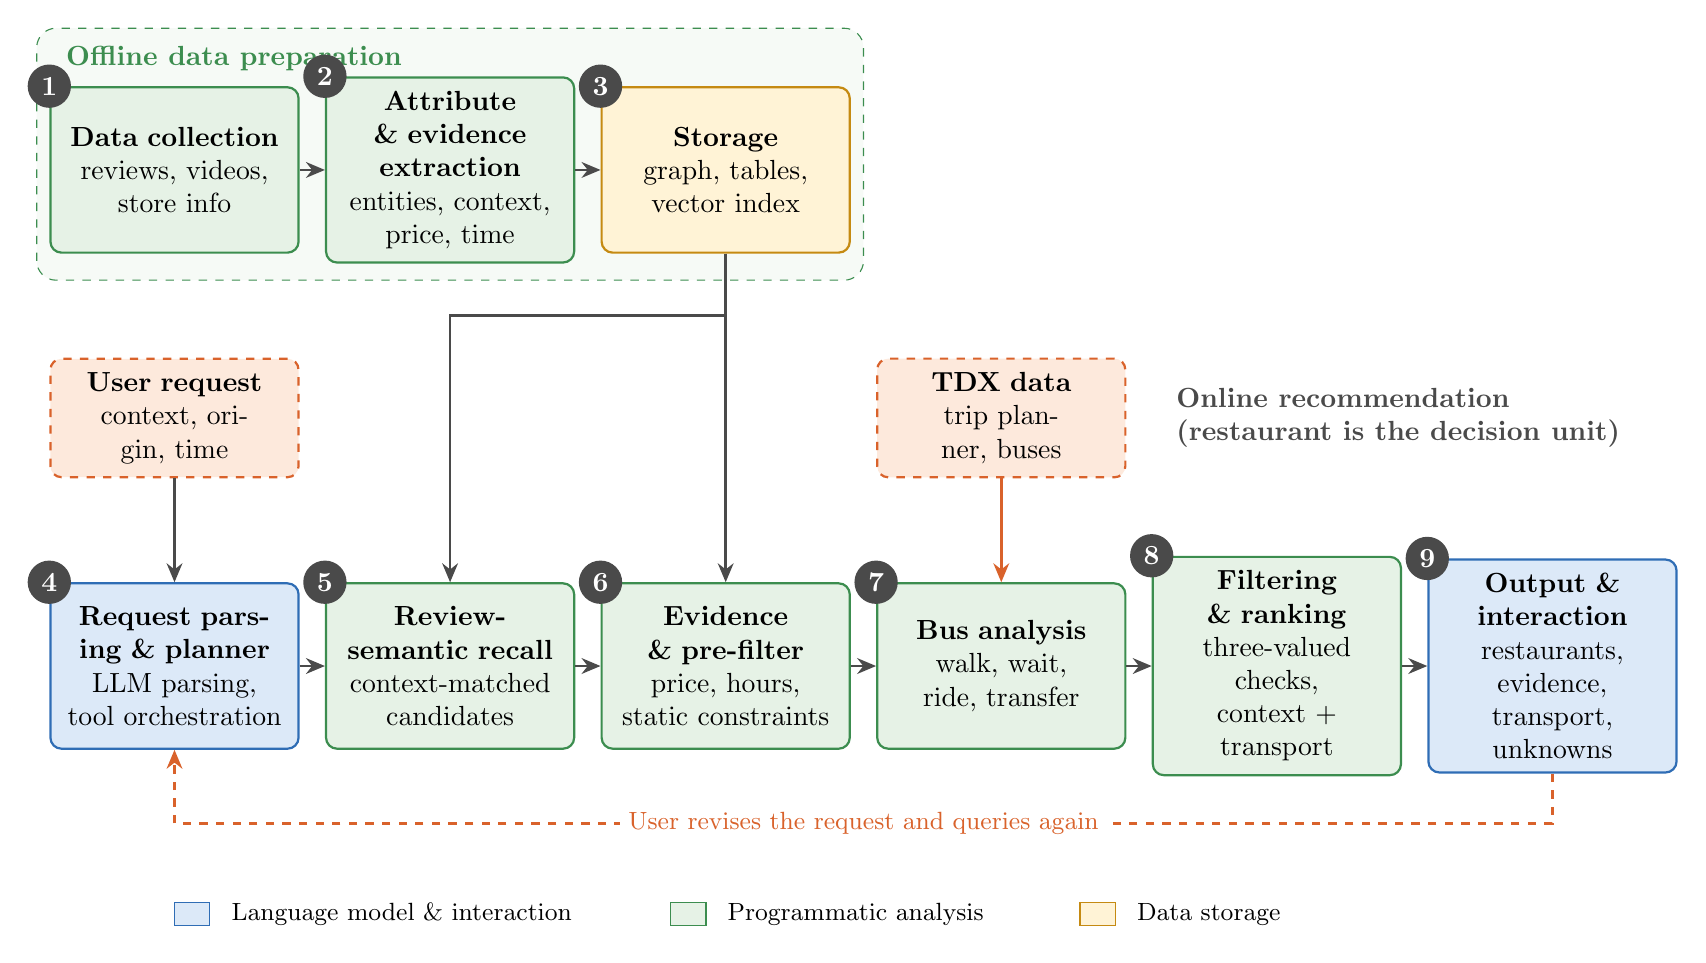
\begin{tikzpicture}[font=\normalsize,>=Stealth,
  box/.style={draw=archProd,fill=archPro,line width=0.8pt,rounded corners=4pt,
    minimum width=3.0cm,minimum height=2.1cm,text width=2.8cm,align=center,inner sep=5pt},
  llm/.style={box,draw=archLLMd,fill=archLLM},
  kb/.style={box,draw=archKBd,fill=archKB},
  src/.style={box,draw=archSrcd,fill=archSrc,dashed,minimum height=1.3cm},
  badge/.style={circle,fill=archGray,text=white,font=\normalsize\bfseries,inner sep=2pt,minimum size=0.55cm},
  arr/.style={-{Stealth[length=2.4mm,width=2mm]},line width=1pt,archGray},
  fb/.style={arr,dashed,archSrcd}]
\fill[archPro!35,draw=archProd,dashed,rounded corners=7pt] (-1.75,4.9) rectangle (8.75,8.1);
\node[anchor=north west,text=archProd,font=\normalsize\bfseries] at (-1.5,8.0) {Offline data preparation};
\node[box] (n1) at (0,6.3) {\textbf{Data collection}\\reviews, videos,\\store info};
\node[box] (n2) at (3.5,6.3) {\textbf{Attribute \& evidence extraction}\\entities, context,\\price, time};
\node[kb] (n3) at (7,6.3) {\textbf{Storage}\\graph, tables,\\vector index};
\node[src] (u) at (0,3.15) {\textbf{User request}\\context, origin, time};
\node[src] (tdx) at (10.5,3.15) {\textbf{TDX data}\\trip planner, buses};
\node[anchor=west,text=archGray,font=\normalsize\bfseries,align=left] at (12.6,3.15) {Online recommendation\\(restaurant is the decision unit)};
\node[llm] (n4) at (0,0) {\textbf{Request parsing \& planner}\\LLM parsing,\\tool orchestration};
\node[box] (n5) at (3.5,0) {\textbf{Review-semantic recall}\\context-matched\\candidates};
\node[box] (n6) at (7,0) {\textbf{Evidence \& pre-filter}\\price, hours,\\static constraints};
\node[box] (n7) at (10.5,0) {\textbf{Bus analysis}\\walk, wait,\\ride, transfer};
\node[box] (n8) at (14,0) {\textbf{Filtering \& ranking}\\three-valued checks,\\context + transport};
\node[llm] (n9) at (17.5,0) {\textbf{Output \& interaction}\\restaurants, evidence,\\transport, unknowns};
\foreach \i in {1,...,9}{\node[badge] at (n\i.north west) {\i};}
\draw[arr] (n1)--(n2);
\draw[arr] (n2)--(n3);
\draw[arr] (u)--(n4);
\foreach \a/\b in {4/5,5/6,6/7,7/8,8/9}{\draw[arr] (n\a.east)--(n\b.west);}
\draw[arr] (n3.south)--(7,4.45)--(3.5,4.45)--(n5.north);
\draw[arr] (n3.south)--(n6.north);
\draw[arr,archSrcd] (tdx.south)--(n7.north);
\draw[fb] (n9.south)--(17.5,-2.0)--(0,-2.0)--(n4.south);
\node[fill=white,inner sep=3pt,text=archSrcd,font=\small] at (8.75,-2.0) {User revises the request and queries again};
\begin{scope}[shift={(0,-3.3)}]
 \draw[archLLMd,fill=archLLM] (0,0) rectangle (0.45,0.3);
 \node[anchor=west,font=\small] at (0.6,0.15) {Language model \& interaction};
 \draw[archProd,fill=archPro] (6.3,0) rectangle (6.75,0.3);
 \node[anchor=west,font=\small] at (6.9,0.15) {Programmatic analysis};
 \draw[archKBd,fill=archKB] (11.5,0) rectangle (11.95,0.3);
 \node[anchor=west,font=\small] at (12.1,0.15) {Data storage};
\end{scope}
\end{tikzpicture}}
\caption{System architecture. Modules 1--3 build restaurant and evidence data offline; modules 4--9 perform request parsing, review-semantic recall, bus analysis, and restaurant recommendation. Transportation is considered before the final ranking.}
\label{fig:architecture}
\end{figure*}

\subsection{Context-Matched Retrieval}
Hybrid recall fuses normalized lexical and dense scores:
\begin{equation}
s_{\mathrm{ret}}(r,q)=\lambda\,\tilde{s}_{\mathrm{BM25}}(r,q)+(1-\lambda)\,\tilde{s}_{\mathrm{vec}}(r,q),\quad 0\le\lambda\le1 .
\end{equation}
Snippet scores are normalized by a fixed rule and aggregated per restaurant before candidate formation, so that restaurants with many near-duplicate reviews do not dominate. The recall size $K$, relevance threshold, normalization, aggregation rule, and $\lambda$ are versioned.

\subsection{Data Sources and Provenance}
Reviews are the core semantic data; video transcripts and comments are supplementary, and the three are labelled as different evidence types. Each text or fact stores a source ID, publication time if available, observation or update time, retrieval time, and validity date. Missing time fields remain empty rather than being filled with crawl time, and a video's publication date does not prove that the prices it mentions are still valid. The Google Places API is used only to map restaurants to place IDs; in accordance with its policy, Places content such as reviews is not pre-fetched or stored~\cite{google_places_policy}. Bus itineraries come from the TDX trip planner, and stops, routes, sub-routes, directions, timetables, and N1 arrival estimates from the TDX bus API~\cite{tdx_planner,tdx_bus}. Records are aligned by identifiers such as RouteUID, never by route name alone.

The knowledge representation distinguishes restaurants, snippets, context attributes, sources, stops, and routes. A restaurant \emph{mentions}-links to snippets, and a snippet \emph{supports}-links to attributes; every support edge carries its source and verification status, and conflicting evidence is kept side by side rather than overwritten. Proximity between a restaurant and a stop only proposes transit candidates; boardability is decided by route and time analysis. Each check is stored as a decision record containing the restaurant ID, plan ID, constraint ID, verdict, reason, evidence IDs, and decision time.

\subsection{Three-Valued Feasibility Checking}
Let $\mathcal{H}(q)$ index the hard constraints of request $q$ and $E$ the available evidence. Each checker returns $h_j(r,p,q,E)\in\{T,F,U\}$: $T$ means satisfied under the available evidence and rules, $F$ means known to be violated, and $U$ means undecidable. The verdicts are aggregated as
\begin{equation}
H(r,p,q,E)=
\begin{cases}
F, & \exists j\in\mathcal{H}(q):\ h_j=F,\\
T, & \forall j\in\mathcal{H}(q):\ h_j=T,\\
U, & \text{otherwise}.
\end{cases}
\end{equation}
The verified itineraries of a restaurant are $\mathcal{P}_T(r,q)=\{p\in\mathcal{P}(r,o,t_{\mathrm{dep}}):H(r,p,q,E)=T\}$. A restaurant enters the verified ranking only if $\mathcal{P}_T(r,q)\neq\emptyset$; pairs with no $F$ but at least one $U$ go to a provisional list. A failed itinerary does not eliminate the restaurant while other itineraries remain. The verdicts describe evidential support, not probabilities; Table~\ref{tab:three_valued} gives the criteria.

\begin{table}[t]
\centering
\caption{Three-Valued Criteria for Hard Constraints}
\label{tab:three_valued}
\footnotesize
\renewcommand{\arraystretch}{1.15}
\setlength{\tabcolsep}{3pt}
\begin{tabular}{@{}L{1.25cm}L{2.2cm}L{2.0cm}L{2.0cm}@{}}
\toprule
\textbf{Constraint} & \textbf{T (pass)} & \textbf{F (fail)} & \textbf{U (unknown)} \\
\midrule
Budget & Upper bound of price range $\le B$ (same unit) & Lower bound $> B$ & Price or unit unknown; range spans $B$ \\
Opening hours & Arrival and departure lie in one valid opening interval & Arrival or meal interval known to violate & Hours, arrival, or meal duration missing \\
Walking & All required legs satisfy the user's limit definition & A leg or the total is known to exceed it & Legs, times, or definition missing \\
Boarding & Stop reached with buffer before bus arrives, within $W_{\max}$ & All allowed buses known to be missed & ETA stale, time base missing, or trip not alignable \\
Transfers & Count $\le N_{\max}$ and every connection holds & Count exceeded or no connection holds & Next leg known only by headway \\
\bottomrule
\end{tabular}
\end{table}

\subsection{Trip and Meal Timeline}
Let $t_{\mathrm{ready}}$ be the time the user reaches the boarding stop including a buffer $b_{\mathrm{board}}$, and $t_{\mathrm{bus}}$ the aligned estimated arrival or departure time. Boarding requires
\begin{equation}\label{eq:boarding}
\begin{aligned}
t_{\mathrm{ready}} &= t_{\mathrm{dep}}+T_{\mathrm{walk\_to\_stop}}+b_{\mathrm{board}},\\
t_{\mathrm{ready}} &\le t_{\mathrm{bus}}\le t_{\mathrm{ready}}+W_{\max}.
\end{aligned}
\end{equation}
For the $i$-th transfer, with previous-leg arrival $a_i$, transfer walk $w_i$, buffer $b_i$, and next departure $d_{i+1}$,
\begin{equation}\label{eq:transfer}
a_i+w_i+b_i\le d_{i+1}.
\end{equation}
A normal status or a non-empty \texttt{EstimateTime} is only an input to this check, not proof of boardability. Countdown values are converted to absolute times only when their reference time is known, and route, sub-route, direction, stop, and stop sequence must be aligned. The arrival and departure times are
\begin{equation}\label{eq:timeline}
\begin{aligned}
t_{\mathrm{arr}}(r,p) &= t_{\mathrm{dep}}+T_{\mathrm{walk}}^{\mathrm{init}}+\textstyle\sum_i\big(T_{\mathrm{wait},i}+T_{\mathrm{ride},i}\big)\\
&\quad+\textstyle\sum_i T_{\mathrm{xfer\_walk},i}+T_{\mathrm{walk}}^{\mathrm{final}},\\
t_{\mathrm{leave}}(r,p) &= t_{\mathrm{arr}}(r,p)+D_{\mathrm{meal}} .
\end{aligned}
\end{equation}
Updated waiting or transfer times propagate to all later events, and segment durations already included in an API itinerary are not added twice. $D_{\mathrm{meal}}$ is taken from the user; a default of 90--120 minutes is shown as an editable assumption. Opening hours are checked over the whole interval $[t_{\mathrm{arr}},t_{\mathrm{leave}}]$, with overnight and split lunch/dinner hours converted to dated intervals. If the last-order time is known it is checked; otherwise only the closing time is checked and the gap is disclosed.

\subsection{Restaurant Ranking}
Transport convenience is computed separately from contextual relevance. For each verified pair,
\begin{equation}\label{eq:ranking}
\begin{aligned}
S(r,p\mid q) &= \alpha s_{\mathrm{sem}}+\beta s_{\mathrm{ctx}}-\gamma c_{\mathrm{food}}-\delta u_{\mathrm{walk}}\\
&\quad-\varepsilon u_{\mathrm{wait}}-\zeta u_{\mathrm{ride\_xfer}}-\eta u_{\mathrm{evid}},\\
p^*(r) &= \arg\max_{p\in\mathcal{P}_T(r,q)} S(r,p\mid q),\\
S_{\mathrm{rest}}(r\mid q) &= S\big(r,p^*(r)\mid q\big),
\end{aligned}
\end{equation}
where $s_{\mathrm{sem}}$ is review--request semantic relevance, $s_{\mathrm{ctx}}$ the source support for the specified context, $c_{\mathrm{food}}$ the meal cost (midpoint of the price range, used only for scoring), $u_{\mathrm{walk}}$ and $u_{\mathrm{wait}}$ the walking and waiting burdens, $u_{\mathrm{ride\_xfer}}$ a fixed combination of separately computed riding and transfer burdens (so that total time cannot hide multiple transfers), and $u_{\mathrm{evid}}$ an evidence-quality cost among already checkable evidence. Cost terms are mapped to $[0,1]$ with fixed truncated linear scaling,
\begin{equation}
\mathcal{N}_{a,b}(x)=\min\!\Big(1,\max\!\Big(0,\tfrac{x-a}{b-a}\Big)\Big),\quad b>a,
\end{equation}
whose bounds are set on development data and not rescaled per candidate set. Weights are non-negative, sum to one, and are frozen before comparison. Keeping only $p^*(r)$ prevents a restaurant with many routes from occupying several result slots. The top three restaurants by $S_{\mathrm{rest}}$ are returned, with ties broken by a fixed ID.

\subsection{Recommendation Algorithm}
Algorithm~\ref{alg:recommend} summarizes the online procedure. A failed route query is recorded separately from a confirmed absence of service, since no response does not prove that no route exists, and ``no verified restaurant'' is decided only after all candidates have been processed. Constraints are never relaxed silently; the user must revise the request explicitly. Explanations are generated from decision records and replaced by a template if they fail a fact check against those records.

\begin{algorithm}[t]
\caption{Context-First Recommendation with Bus Analysis}
\label{alg:recommend}
\footnotesize
\begin{algorithmic}[1]
\Require query $Q$, origin $o$, departure time $t_{\mathrm{dep}}$
\Ensure restaurants $R$, bus plans, explanations, provisional items
\State $q\gets$ \Call{ParseWithSchema}{$Q,o,t_{\mathrm{dep}}$}
\If{required fields missing or invalid} \Return \Call{AskOrExplain}{$q$} \EndIf
\State $C\gets$ \Call{RetrieveContextMatched}{$q$}; $C\gets$ \Call{Dedup}{$C$}
\If{$C=\emptyset$} \Return \Call{ExplainNoMatch}{} \EndIf
\State $E\gets$ \Call{RetrieveEvidence}{$C$}
\State $C\gets$ \Call{RemoveStaticFailures}{$C,E$}; $C\gets$ \Call{TopK}{$C$}
\State $V,P_U,\mathit{Rec}\gets\emptyset$
\For{each restaurant $r\in C$}
  \State $(\mathcal{P},\mathit{st})\gets$ \Call{GetBusPlans}{$o,r,t_{\mathrm{dep}}$}
  \If{$\mathit{st}$ yields no usable plan}
    \State record failure or unknown in $\mathit{Rec}$; \textbf{continue}
  \EndIf
  \For{each plan $p\in\mathcal{P}$}
    \State $d\gets$ \Call{FetchAndAlignBusData}{$p$}
    \State $\tau\gets$ \Call{BuildTimeline}{$r,p,q,d$}
    \State $h\gets$ \Call{CheckConstraints}{$r,p,\tau,E$}
    \State append decision record to $\mathit{Rec}$
    \If{$\exists F\in h$} \textbf{continue}
    \ElsIf{$\exists U\in h$} add $(r,p)$ to $P_U$
    \Else\ add $(r,p,S(r,p\mid q))$ to $V$
    \EndIf
  \EndFor
\EndFor
\State $V^*\gets$ \Call{BestPlanPerRestaurant}{$V$}
\State $R\gets$ top three of \Call{StableSort}{$V^*$}
\If{$R=\emptyset$} \Return \Call{NoVerifiedResult}{$P_U,\mathit{Rec}$} \EndIf
\State $X\gets$ \Call{GenerateFromRecords}{$R,\mathit{Rec}$}
\If{$X$ fails fact check} $X\gets$ \Call{Template}{$R,\mathit{Rec}$} \EndIf
\State \Return $R$, plans, $X$, $P_U$, $\mathit{Rec}$
\end{algorithmic}
\end{algorithm}

% -----------------------------------------------------------------------------
\section{Evaluation Protocol}\label{sec:eval}

All quantities in this section are planned values; the experiments have not yet been run.

\subsection{Data and Annotation}
The evaluation targets Taichung City; the covered districts and bus routes will be fixed after a data audit. Restaurant data are extracted from transcripts of selected food-review videos (names, locations, dishes, price levels, and opinions), using the video's publication date as the data time, plus viewer comments; the selection criteria for channels, period, and districts will be fixed and published before collection. About 100 restaurants are planned, depending on what can be extracted. Ground truth for opening hours and prices comes from official store information or sampled on-site or phone verification.

Queries are generated from templates and by hand and stratified by constraint type (budget, opening hours, walking limit, direct vs. one-transfer trips, dietary preference) and meal period (lunch, dinner, late night), so that hard-constraint violations actually occur in each stratum. We plan a pilot set of 50 queries and a main set of 200 (60 for tuning, 140 for testing), with the size revisited by a power analysis based on pilot violation rates. Hard-constraint labels are derived from data sources and live checks; only preference relevance is labelled independently by two annotators, and inter-annotator agreement is reported.

\subsection{Baselines and Ablations}
Table~\ref{tab:baselines} maps each research question to its comparison. The graph-versus-relational comparison (exploratory) must use identical facts and rules, since removing the graph together with its facts would not isolate the graph's effect.

\begin{table}[t]
\centering
\caption{Research Questions, Comparisons, and Metrics}
\label{tab:baselines}
\footnotesize
\renewcommand{\arraystretch}{1.15}
\setlength{\tabcolsep}{3pt}
\begin{tabular}{@{}L{0.75cm}L{3.2cm}L{3.55cm}@{}}
\toprule
\textbf{RQ} & \textbf{Comparison} & \textbf{Metrics} \\
\midrule
RQ1 & Keyword vs.\ vector vs.\ hybrid recall & Recall@$K$, MRR, nDCG (final choice fixed in pilot) \\
RQ2 & Context-first ranking with bus analysis vs.\ semantic ranking with route appended & Violation rate, total travel and waiting time, share of rankings changed by transport \\
RQ3 & Full evidence checking vs.\ direct LLM ranking & Violation rate, unsupported-claim rate, coverage, abstention rate \\
RQ4 & Timeline at arrival vs.\ opening check at departure; with vs.\ without N1 arrival checks & Closed-on-arrival rate by meal period; missed boarding/transfer rate; accuracy of $U$ labels (field ground truth) \\
Expl. & Knowledge graph vs.\ relational tables (same facts) & Query correctness, evidence completeness \\
\bottomrule
\end{tabular}
\end{table}

\subsection{Metrics}
The \emph{violation rate} is the number of plans claimed feasible that violate at least one constraint, divided by all plans claimed feasible. The \emph{unsupported-claim rate} is the number of plans with insufficient required evidence that are nevertheless claimed to pass, over the same denominator. \emph{Coverage} is the fraction of test queries that return at least one verified plan and is always reported alongside the violation rate, so that a low error rate cannot be bought by abstaining; both rates are marked not applicable when there is no output. Queries without any relevant restaurant are reported separately rather than given a perfect nDCG.

\subsection{Bus Data Collection and Field Validation}
The N1 arrival-estimate endpoint will be polled at fixed intervals for one to two weeks on selected routes, within the TDX rate limits, to measure the share of stops with live estimates, the distribution of status codes, missing values, and update latency. About 30 real trips will be taken to record whether the recommended bus arrives within the predicted window and whether transfers connect; these trips provide the only ground truth for actual arrivals.

\subsection{Statistics and Reproducibility}
Systems are compared pairwise on the same queries with 95\% bootstrap confidence intervals and Holm correction for multiple comparisons; negative results are reported as well. Paraphrases and template instances of the same scenario are grouped before splitting, and multiple plans for one query are not treated as independent samples. Code, model and embedding versions, prompts, schemas, weights, random seeds, split lists, and raw responses are archived, and test queries are never used to tune weights or labels.

% Results will be added here after the experiments are completed:
% \section{Results}
% \subsection{RQ1: Context Retrieval}
% \subsection{RQ2: Effect of Bus Accessibility on Ranking}
% \subsection{RQ3: Three-Valued Checking}
% \subsection{RQ4: Timeline Checking}

% -----------------------------------------------------------------------------
\section{Discussion and Limitations}\label{sec:discussion}

\textbf{Timetables versus live data.} Timetables provide service days and planned connections, while live data reflect observable delays. The replanning study of Abuaisha \emph{et al.} supports the value of live updates but relies on synthetic delays~\cite{bus_dynamic_replanning}, so it cannot determine coverage, update intervals, or query frequency for Taichung. We therefore form candidates from timetables and the trip planner, check boarding against live evidence where available, and record the time base used.

\textbf{Travel time versus transfer reliability.} Ranking by a single predicted arrival may favour plans with tight transfers, yet delay distributions are wide~\cite{bus_delay_uncertainty}. Larger buffers protect connections but may exclude boardable plans or lengthen trips, and existing evidence does not justify a universal buffer. Buffers are thus versioned parameters, and passing a check is never presented as a success probability.

\textbf{LLM parsing risk.} Even with correct downstream code, a misparsed budget unit or date leads the system to verify the wrong constraint. Parsed fields therefore keep their mapping to the original wording, and ambiguities that affect hard constraints trigger clarification.

\textbf{Scope.} Data from food videos carry selection bias, and transcript extraction may contain errors; the restaurant set is limited because Places content cannot be stored. Arrival estimates are not guaranteed to be accurate and may not cover the next leg after a transfer, in which case only headway is known and the verdict is $U$. The study covers only Taichung urban buses and excludes reservations, queues, and other transport modes, so results from a single city with manual annotation do not support cross-city conclusions. All expected improvements are hypotheses, and results reported elsewhere do not establish effectiveness in this domain.

% -----------------------------------------------------------------------------
\section{Conclusion and Future Work}\label{sec:conclusion}

We presented a context-aware restaurant recommendation agent that recalls occasion-matched restaurants from review semantics and then uses Taichung bus walking, waiting, riding, and transfer conditions to filter and rank them before the final decision. Hard constraints are checked in code over a complete trip-and-meal timeline with three-valued verdicts, which separates infeasible options from those lacking evidence, and explanations are generated from traceable decision records. We also specified an evaluation protocol with baselines, ablations, coverage-aware error metrics, and paired statistical tests. Future work includes executing this protocol, monitoring trips after departure with delay-triggered re-ranking and alternative-restaurant suggestions, return-trip checking after the meal, calibration of arrival-estimate errors once enough observed arrivals are collected, and extension to other transport modes.

% -----------------------------------------------------------------------------
\bibliographystyle{IEEEtran}
\bibliography{bib/ieee_paper}

\end{document}
